\title{Worldview Modeling - Inspiration}
\author{Ryan Spangler}
\date{\today}

\documentclass[12pt]{article}

\usepackage{graphicx}

\setcounter{secnumdepth}{0}

\begin{document}
\maketitle

\section{Modeling Neural Dynamics}

My current interests lie in cellular and neural electrical and informational dynamics.  I am most interested in how it is possible for something to be alive?  The entire process is baffling and amazing.  A huge group of independently acting, loosely coordinated molecules manages to hold itself together despite a host of hostile and unpredictable forces trying to tear it apart?  And not just that it succeeds, but that it can't seem to help it.  A living thing brings all resources to bear to maintain its existence.  Of course, it does not always succeed, but if you include the propagation by reproduction life is wildly successful.

The entire fabric of an organism is dedicated to the maintenance and propagation of that very fabric which is doing the maintaining!  I think this circular causality is actually the essential ingredient in a thing being living.  Anything with the same circular causality can be considered alive, no matter what the medium it is manifest in.  

This circular causality is elusive and seemingly paradoxical.  I will attempt to make sense of this, and cast it in terms that can be modelled somehow.   

Beyond merely (!) living, how can living things think?  What is this process of experience?  How can this mass of goo comprehend its environment?  Do cells think?  It could be that if something is living, it has some measure of experience, so that even cells perceive to some degree.  One idea is to identify how portions of the stochastic molecular mechanisms of the cell are actually performing the same function as a nervous system, which is to correlate experience with perception to make predictions and guide action and response to novel situations.  Learning about both in depth will facilitate connections that illuminate general principles of living things.

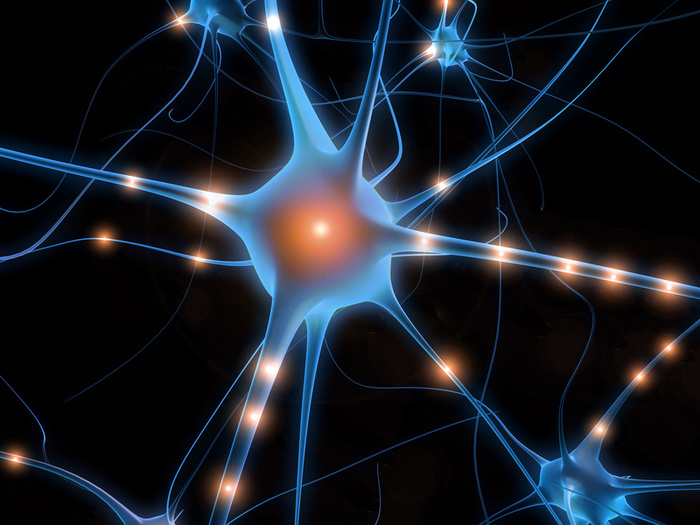
\includegraphics[scale=2.0]{1077neuron.jpg}

\vspace{15pt}

In the immediate term, I would like to make a model of neural or cellular prediction (relying on present biophysical knowledge), a simple and composable unit that reconciles expectations with perception using harmonic resonance.  And then if I make it that far, start composing them in heirarchies and provide an environment for operational closure (ie some link between actions and perceptions (which we call the world)).

\end{document}
